\documentclass[tikz]{standalone}
\usetikzlibrary{patterns}
\usetikzlibrary{shapes,arrows}
\usetikzlibrary{decorations.pathreplacing, positioning}
\definecolor{greengreen}{rgb}{0.0, 0.42, 0.24}
\definecolor{calpolypomonagreen}{rgb}{0.12, 0.3, 0.17}
\definecolor{forestgreen}{rgb}{0.13, 0.55, 0.13}

\begin{document}
\noindent
  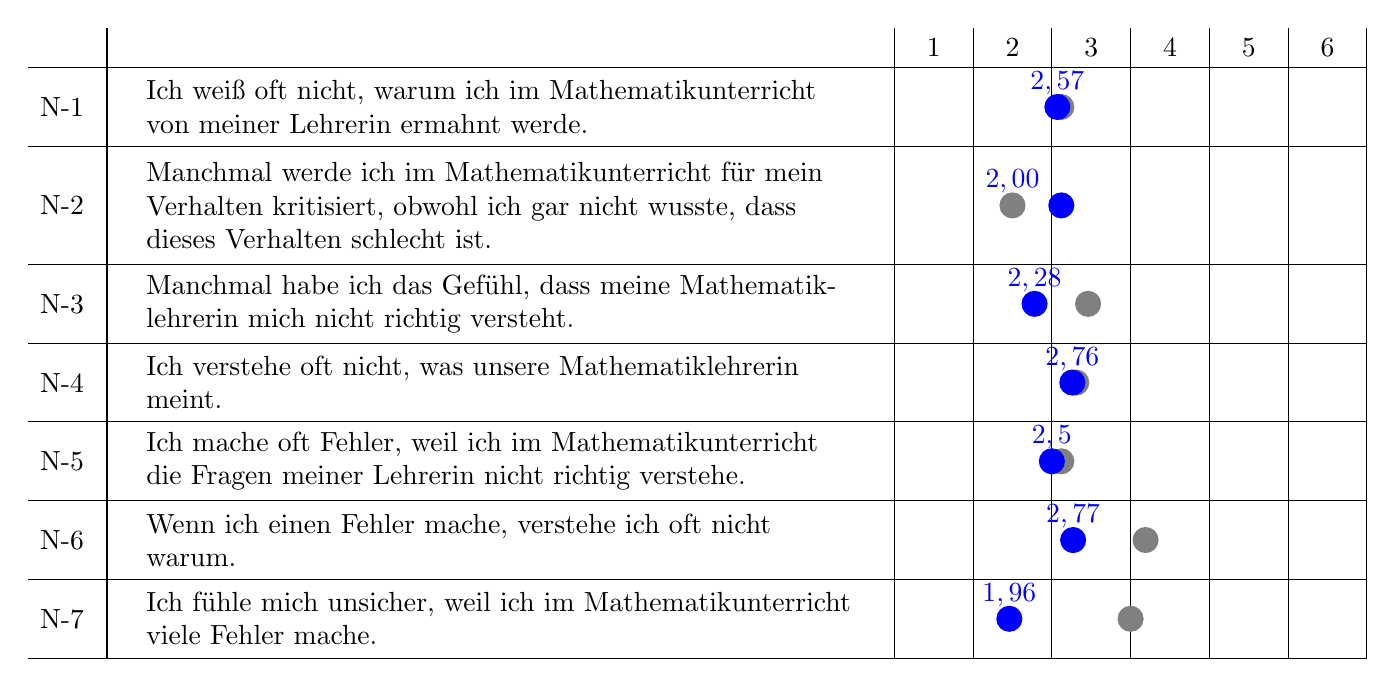
\begin{tikzpicture}

    \foreach \y in {0,1,2.5,3.5,4.5,5.5,6.5,7.5}
        \draw (-1, 0 - \y) -- (16, 0 - \y);
    \foreach \x in {0,10,11,12,13,14,15,16}
        \draw (0 + \x, 0.5) -- (0 + \x, - 7.5);
    
    \node at (10.5, 0.25) {$1$};
    \node at (11.5, 0.25) {$2$};
    \node at (12.5, 0.25) {$3$};
    \node at (13.5, 0.25) {$4$};
    \node at (14.5, 0.25) {$5$};
    \node at (15.5, 0.25) {$6$};


    \node[thick, align=left, text width=1cm] at (-0.35, -0.5) {N-1};
    \node[thick, align=left, text width=9cm] at (5, -0.5) {Ich weiß oft nicht, warum ich im Mathematikunterricht von meiner Lehrerin ermahnt werde.};
    \node[thick, circle, fill=gray, minimum width=0.25] (1) at (9.5 + 2.62, -0.5) {};
    \node[thick, blue] at (9.5 + 2.57, -0.2) {$2,57$};
    \node[thick, circle, fill=blue, minimum width=0.25] (1) at (9.5 + 2.57, -0.5) {};


    \node[thick, align=left, text width=1cm] at (-0.35, -1.75) {N-2};
    \node[thick, align=left, text width=9cm] at (5, -1.75) {Manchmal werde ich im Mathematikunterricht für mein Verhalten kritisiert, obwohl ich gar nicht wusste, dass dieses Verhalten schlecht ist.};
    \node[thick, circle, fill=gray, minimum width=0.25] (2) at (9.5 + 2.00, -1.75) {};
    \node[thick, blue] at (9.5 + 2, -1.45) {$2,00$};
    \node[thick, circle, fill=blue, minimum width=0.25] (1) at (9.5 + 2.62, -1.75) {};


    \node[thick, align=left, text width=1cm] at (-0.35, -3) {N-3};
    \node[thick, align=left, text width=9cm] at (5, -3) {Manchmal habe ich das Gefühl, dass meine Mathematiklehrerin mich nicht richtig versteht.};
    \node[thick, circle, fill=gray, minimum width=0.25] (3) at (9.5 + 2.96, -3) {};
    \node[thick, blue] at (9.5 + 2.28, -2.7) {$2,28$};
    \node[thick, circle, fill=blue, minimum width=0.25] (1) at (9.5 + 2.28, -3) {};


    \node[thick, align=left, text width=1cm] at (-0.35, -4) {N-4};
    \node[thick, align=left, text width=9cm] at (5, -4) {Ich verstehe oft nicht, was unsere Mathematiklehrerin meint.};
    \node[thick, circle, fill=gray, minimum width=0.25] (4) at (9.5 + 2.81, -4) {};
    \node[thick, blue] at (9.5 + 2.76, -3.7) {$2,76$};
    \node[thick, circle, fill=blue, minimum width=0.25] (1) at (9.5 + 2.76, -4) {};


    \node[thick, align=left, text width=1cm] at (-0.35, -5) {N-5};
    \node[thick, align=left, text width=9cm] at (5, -5) {Ich mache oft Fehler, weil ich im Mathematikunterricht die Fragen meiner Lehrerin nicht richtig verstehe.};
    \node[thick, circle, fill=gray, minimum width=0.25] (5) at (9.5 + 2.62, -5) {};
    \node[thick, blue] at (9.5 + 2.5, -4.7) {$2,5$};
    \node[thick, circle, fill=blue, minimum width=0.25] (1) at (9.5 + 2.5, -5) {};


    \node[thick, align=left, text width=1cm] at (-0.35, -6) {N-6};
    \node[thick, align=left, text width=9cm] at (5, -6) {Wenn ich einen Fehler mache, verstehe ich oft nicht warum.};
    \node[thick, circle, fill=gray, minimum width=0.25] (6) at (9.5 + 3.69, -6) {};
    \node[thick, blue] at (9.5 + 2.77, -5.7) {$2,77$};
    \node[thick, circle, fill=blue, minimum width=0.25] (1) at (9.5 + 2.77, -6) {};


    \node[thick, align=left, text width=1cm] at (-0.35, -7) {N-7};
    \node[thick, align=left, text width=9cm] at (5, -7) {Ich fühle mich unsicher, weil ich im Mathematikunterricht viele Fehler mache.};
    \node[thick, circle, fill=gray, minimum width=0.25] (7) at (9.5 + 3.5, -7) {};
    \node[thick, blue] at (9.5 + 1.96, -6.7) {$1,96$};
    \node[thick, circle, fill=blue, minimum width=0.25] (1) at (9.5 + 1.96, -7) {};


    %\draw[color=blue, thick] (1) to (2) to (3) to (4) to (5);

  \end{tikzpicture}%
\end{document}
